\subsection{suEXEC}

\begin{frame}
  \frametitle{Serving static content}
  \begin{itemize}
  \item The \texttt{apache} user does not have permission to read the
    user's files directly.
  \item Both static and dynamic content is served through suEXEC.
  \end{itemize}
\end{frame}

\begin{frame}[fragile,t]
  \begin{enumerate}
  \item \texttt{/etc/httpd/conf.d/execsys.conf} is configured to serve
    static content with the \texttt{cgi-script} handler.
  \end{enumerate}
\begin{footnotesize}
\begin{semiverbatim}
<FilesMatch ``(?i)\\.(cgi|exe|php|pl|py|scm)$''>
        SetHandler cgi-script
        Options +ExecCGI
</FilesMatch>
<FilesMatch ``(?i)\\.(avi|css|doc|docm|docx|\ldots|zip)$''>
        SetHandler cgi-script
        Options +ExecCGI
</FilesMatch>
\ldots
\end{semiverbatim}
\end{footnotesize}
\end{frame}

\begin{frame}[fragile,t]
  \begin{enumerate}
    \addtocounter{enumi}{2}
  \item \texttt{httpd/support/suexec.c} is modified to dispatch static
    content to \texttt{/usr/local/bin/static-cat}.
  \end{enumerate}
\begin{footnotesize}
\begin{semiverbatim}
+#define STATIC_CAT_PATH "/usr/bin/static-cat"
+static const char *static_extensions[] = \{
+    "html",
+    "css",
+    \ldots
+\}
+
 int main(int argc, char *argv[])
 \{ \ldots
+
+    if (is_static_extension(cmd)) \{
+        if (setenv("PATH_TRANSLATED", cmd, 1) != 0) \{
+            log_err("setenv failed\\n");
+            exit(255);
+        \}
+        execl(STATIC_CAT_PATH, STATIC_CAT_PATH, (const char *)NULL);
+        log_err("(%d)%s: static-cat exec failed (%s)\\n", errno,
+                strerror(errno), STATIC_CAT_PATH);
+        exit(255);
+    \}
\end{semiverbatim}
\end{footnotesize}
\end{frame}

{
  \usebackgroundtemplate{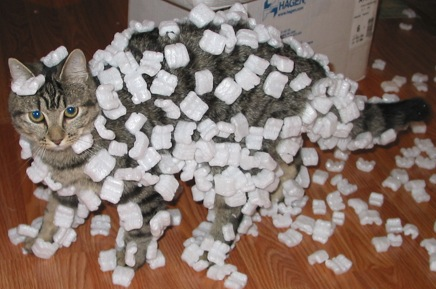
\includegraphics[keepaspectratio=true,height=\paperheight,width=\paperwidth]{static-cat.jpg}}
  \setbeamertemplate{navigation symbols}{}
  \begin{frame}[plain]
  \end{frame}
}
